\documentclass[../main.tex]{subfiles}

\begin{document}
\section{1D Fields}
While boxplots were designed to visualize discrete observations, often there
are no discrete observations and instead the `observation` is a timeseries
curve (where the connections are as important as the individual points) or
spatial region. Understanding the distributions of functional observations
often relies first ordering the functions such that there's some measure of how
close these functions are to each other--functional depth\cite{febrero2007},
bivariate score depth\cite{hyndman2009}, and
bivariate kernel density estimation\cite{scott1992} are some examples. This
ordering then yields functional analogs to median and other percentile
metrics. For small values, the ordered curves can then be colored based on the
ordering metric \cite{hyndman2009}, but this method is unweildy for larger
ensembles.

\subsection{Univariate Observations}

\begin{figure}
  %%\includegraphics{funcbaghdr}
  \label{fig:funcbag}
\end{figure}
Instead, Hyndmand and Shang proposed functional versions of the bag and HDR
plots\cite{hyndman2009}, as shown in Figure~\ref{fig:funcbag}. In these graphs,
what was traditionally the box part of a box plot is now a region bounded by
the curves (obtained by using one of the previously mentioned ordering
metrics). The median curve is defined as a blackline and the exceptional
outlines are shown. By using regions defined by the curves, the functional bag
and HDR plots display the variance in the ensembles while simulatanously
flattening the similaraties so that the outliers are strongly highlighted. The
HDR method better highlights outliers closer to the median, whereas the bagplot
method better highlights the outliers outside the envelopes of functions.



The functional boxplot was developed to describe the distributional nature of
functional data\cite{sun2011}. \textbf{expand this section with discusson of
  Sun's paper}


\begin{figure}
  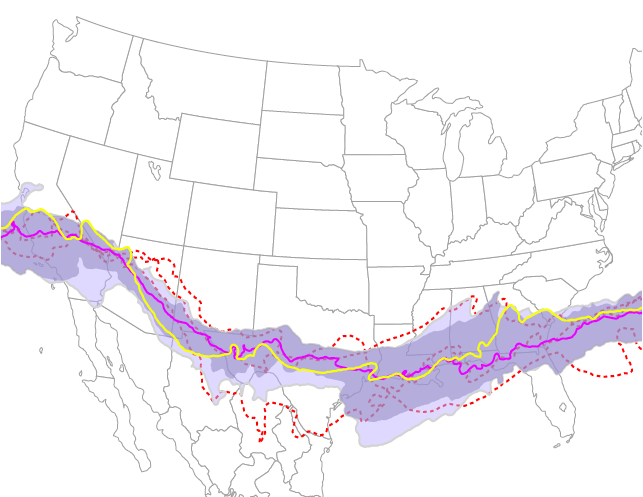
\includegraphics[width=.75\linewidth]{contour_weather}
  \caption{\label{fig:countour}}
\end{figure}
While functional bag, box, and HDR plots all show outliers, each method is most
successful visualizing a specific type of outlier. Countour
boxplots\cite{whitaker2013} aim instead to capture the variablity of the
uncertainity via a band depth ordering metric. Each ensemble members band depth
is computed as sum of the probabilities that the observations in any given
ensemble fall within the max-min envelope defined by any two other
ensembles. The bands are then sorted by band depth such that the median is the
ensemble with about 50\% of its members withen all envelopes formed by other
bands (so most centered). Outer bands are chosen according to the task at
hand. In \cite{whitaker2013}, they apply the countour boxplots to temperature
visualizations. The authors argue that countour boxplots are an improved visual
idiom over the traditional spagehtti plots (%insert citation for them...)
because the spagehetti plots get nosy as the number of plots increase
and so it's hard to tease out specific patterns. Instead in
Figure~\ref{fig:countour}, the authorsremove most of the bands and instead visualize an outlier envelope(light gray)
and a more central envelope(dark gray). It retains much of the information of
the spagethhit, but removes the visual noise of the lines.



\subsection{Bivariate Observations}
%%hurricane tracks (x+y dept) 

surface map, functional correlations, planes?

\subsection{Multivariate Observations}
LDA, CCA, 
PLS, functional PCA

